% Created by tikzDevice version 0.10.1 on 2016-09-01 16:04:14
% !TEX encoding = UTF-8 Unicode
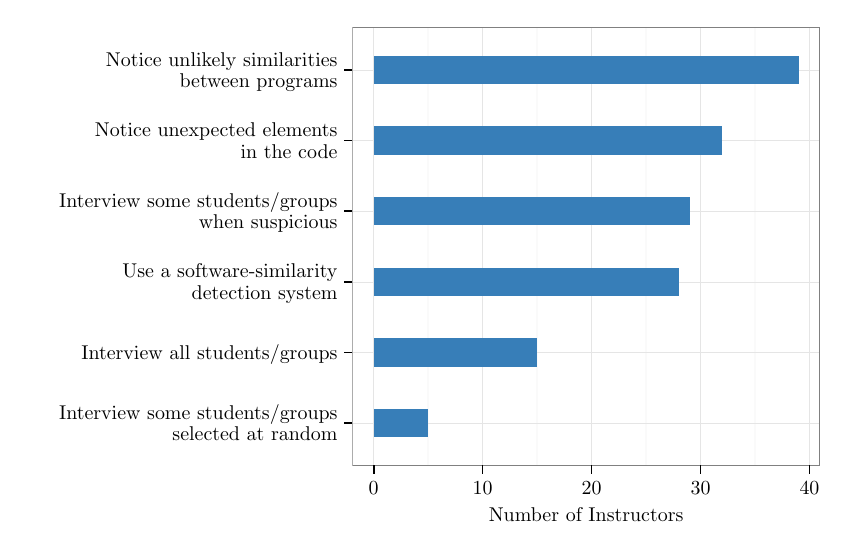
\begin{tikzpicture}[x=1pt,y=1pt]
\definecolor{fillColor}{RGB}{255,255,255}
\path[use as bounding box,fill=fillColor,fill opacity=0.00] (0,0) rectangle (289.08,180.67);
\begin{scope}
\path[clip] (  0.00,  0.00) rectangle (289.08,180.67);
\definecolor{drawColor}{RGB}{255,255,255}
\definecolor{fillColor}{RGB}{255,255,255}

\path[draw=drawColor,line width= 0.6pt,line join=round,line cap=round,fill=fillColor] (  0.00,  0.00) rectangle (289.08,180.68);
\end{scope}
\begin{scope}
\path[clip] (117.36, 22.52) rectangle (286.23,180.67);
\definecolor{fillColor}{RGB}{255,255,255}

\path[fill=fillColor] (117.36, 22.52) rectangle (286.23,180.67);
\definecolor{drawColor}{gray}{0.98}

\path[draw=drawColor,line width= 0.6pt,line join=round] (144.72, 22.52) --
	(144.72,180.67);

\path[draw=drawColor,line width= 0.6pt,line join=round] (184.08, 22.52) --
	(184.08,180.67);

\path[draw=drawColor,line width= 0.6pt,line join=round] (223.45, 22.52) --
	(223.45,180.67);

\path[draw=drawColor,line width= 0.6pt,line join=round] (262.81, 22.52) --
	(262.81,180.67);
\definecolor{drawColor}{gray}{0.90}

\path[draw=drawColor,line width= 0.2pt,line join=round] (117.36, 37.82) --
	(286.23, 37.82);

\path[draw=drawColor,line width= 0.2pt,line join=round] (117.36, 63.33) --
	(286.23, 63.33);

\path[draw=drawColor,line width= 0.2pt,line join=round] (117.36, 88.84) --
	(286.23, 88.84);

\path[draw=drawColor,line width= 0.2pt,line join=round] (117.36,114.35) --
	(286.23,114.35);

\path[draw=drawColor,line width= 0.2pt,line join=round] (117.36,139.86) --
	(286.23,139.86);

\path[draw=drawColor,line width= 0.2pt,line join=round] (117.36,165.37) --
	(286.23,165.37);

\path[draw=drawColor,line width= 0.2pt,line join=round] (125.03, 22.52) --
	(125.03,180.67);

\path[draw=drawColor,line width= 0.2pt,line join=round] (164.40, 22.52) --
	(164.40,180.67);

\path[draw=drawColor,line width= 0.2pt,line join=round] (203.76, 22.52) --
	(203.76,180.67);

\path[draw=drawColor,line width= 0.2pt,line join=round] (243.13, 22.52) --
	(243.13,180.67);

\path[draw=drawColor,line width= 0.2pt,line join=round] (282.50, 22.52) --
	(282.50,180.67);
\definecolor{fillColor}{RGB}{55,126,184}

\path[fill=fillColor] (125.03, 32.72) rectangle (144.72, 42.92);

\path[fill=fillColor] (125.03, 58.23) rectangle (184.08, 68.43);

\path[fill=fillColor] (125.03, 83.74) rectangle (235.26, 93.94);

\path[fill=fillColor] (125.03,109.25) rectangle (239.19,119.45);

\path[fill=fillColor] (125.03,134.76) rectangle (251.00,144.96);

\path[fill=fillColor] (125.03,160.27) rectangle (278.56,170.47);
\definecolor{drawColor}{gray}{0.50}

\path[draw=drawColor,line width= 0.6pt,line join=round,line cap=round] (117.36, 22.52) rectangle (286.23,180.67);
\end{scope}
\begin{scope}
\path[clip] (  0.00,  0.00) rectangle (289.08,180.67);
\definecolor{drawColor}{RGB}{0,0,0}

\node[text=drawColor,anchor=base east,inner sep=0pt, outer sep=0pt, scale=  0.72] at (111.96, 39.23) {Interview some students/groups};

\node[text=drawColor,anchor=base east,inner sep=0pt, outer sep=0pt, scale=  0.72] at (111.96, 31.46) {selected at random};

\node[text=drawColor,anchor=base east,inner sep=0pt, outer sep=0pt, scale=  0.72] at (111.96, 60.85) {Interview all students/groups};

\node[text=drawColor,anchor=base east,inner sep=0pt, outer sep=0pt, scale=  0.72] at (111.96, 90.25) {Use a software-similarity};

\node[text=drawColor,anchor=base east,inner sep=0pt, outer sep=0pt, scale=  0.72] at (111.96, 82.47) {detection system};

\node[text=drawColor,anchor=base east,inner sep=0pt, outer sep=0pt, scale=  0.72] at (111.96,115.76) {Interview some students/groups};

\node[text=drawColor,anchor=base east,inner sep=0pt, outer sep=0pt, scale=  0.72] at (111.96,107.98) {when suspicious};

\node[text=drawColor,anchor=base east,inner sep=0pt, outer sep=0pt, scale=  0.72] at (111.96,141.27) {Notice unexpected elements};

\node[text=drawColor,anchor=base east,inner sep=0pt, outer sep=0pt, scale=  0.72] at (111.96,133.49) {in the code};

\node[text=drawColor,anchor=base east,inner sep=0pt, outer sep=0pt, scale=  0.72] at (111.96,166.78) {Notice unlikely similarities};

\node[text=drawColor,anchor=base east,inner sep=0pt, outer sep=0pt, scale=  0.72] at (111.96,159.00) {between programs};
\end{scope}
\begin{scope}
\path[clip] (  0.00,  0.00) rectangle (289.08,180.67);
\definecolor{drawColor}{RGB}{0,0,0}

\path[draw=drawColor,line width= 0.6pt,line join=round] (114.36, 37.82) --
	(117.36, 37.82);

\path[draw=drawColor,line width= 0.6pt,line join=round] (114.36, 63.33) --
	(117.36, 63.33);

\path[draw=drawColor,line width= 0.6pt,line join=round] (114.36, 88.84) --
	(117.36, 88.84);

\path[draw=drawColor,line width= 0.6pt,line join=round] (114.36,114.35) --
	(117.36,114.35);

\path[draw=drawColor,line width= 0.6pt,line join=round] (114.36,139.86) --
	(117.36,139.86);

\path[draw=drawColor,line width= 0.6pt,line join=round] (114.36,165.37) --
	(117.36,165.37);
\end{scope}
\begin{scope}
\path[clip] (  0.00,  0.00) rectangle (289.08,180.67);
\definecolor{drawColor}{RGB}{0,0,0}

\path[draw=drawColor,line width= 0.6pt,line join=round] (125.03, 19.52) --
	(125.03, 22.52);

\path[draw=drawColor,line width= 0.6pt,line join=round] (164.40, 19.52) --
	(164.40, 22.52);

\path[draw=drawColor,line width= 0.6pt,line join=round] (203.76, 19.52) --
	(203.76, 22.52);

\path[draw=drawColor,line width= 0.6pt,line join=round] (243.13, 19.52) --
	(243.13, 22.52);

\path[draw=drawColor,line width= 0.6pt,line join=round] (282.50, 19.52) --
	(282.50, 22.52);
\end{scope}
\begin{scope}
\path[clip] (  0.00,  0.00) rectangle (289.08,180.67);
\definecolor{drawColor}{RGB}{0,0,0}

\node[text=drawColor,anchor=base,inner sep=0pt, outer sep=0pt, scale=  0.72] at (125.03, 12.16) {0};

\node[text=drawColor,anchor=base,inner sep=0pt, outer sep=0pt, scale=  0.72] at (164.40, 12.16) {10};

\node[text=drawColor,anchor=base,inner sep=0pt, outer sep=0pt, scale=  0.72] at (203.76, 12.16) {20};

\node[text=drawColor,anchor=base,inner sep=0pt, outer sep=0pt, scale=  0.72] at (243.13, 12.16) {30};

\node[text=drawColor,anchor=base,inner sep=0pt, outer sep=0pt, scale=  0.72] at (282.50, 12.16) {40};
\end{scope}
\begin{scope}
\path[clip] (  0.00,  0.00) rectangle (289.08,180.67);
\definecolor{drawColor}{RGB}{0,0,0}

\node[text=drawColor,anchor=base,inner sep=0pt, outer sep=0pt, scale=  0.72] at (201.80,  2.40) {Number of Instructors};
\end{scope}
\end{tikzpicture}
